\section{Capturarea și înțelegerea imaginilor}\label{understanding_spec}

% \begin{wrapfigure}{R}{0.3\textwidth}
%   \centering
%   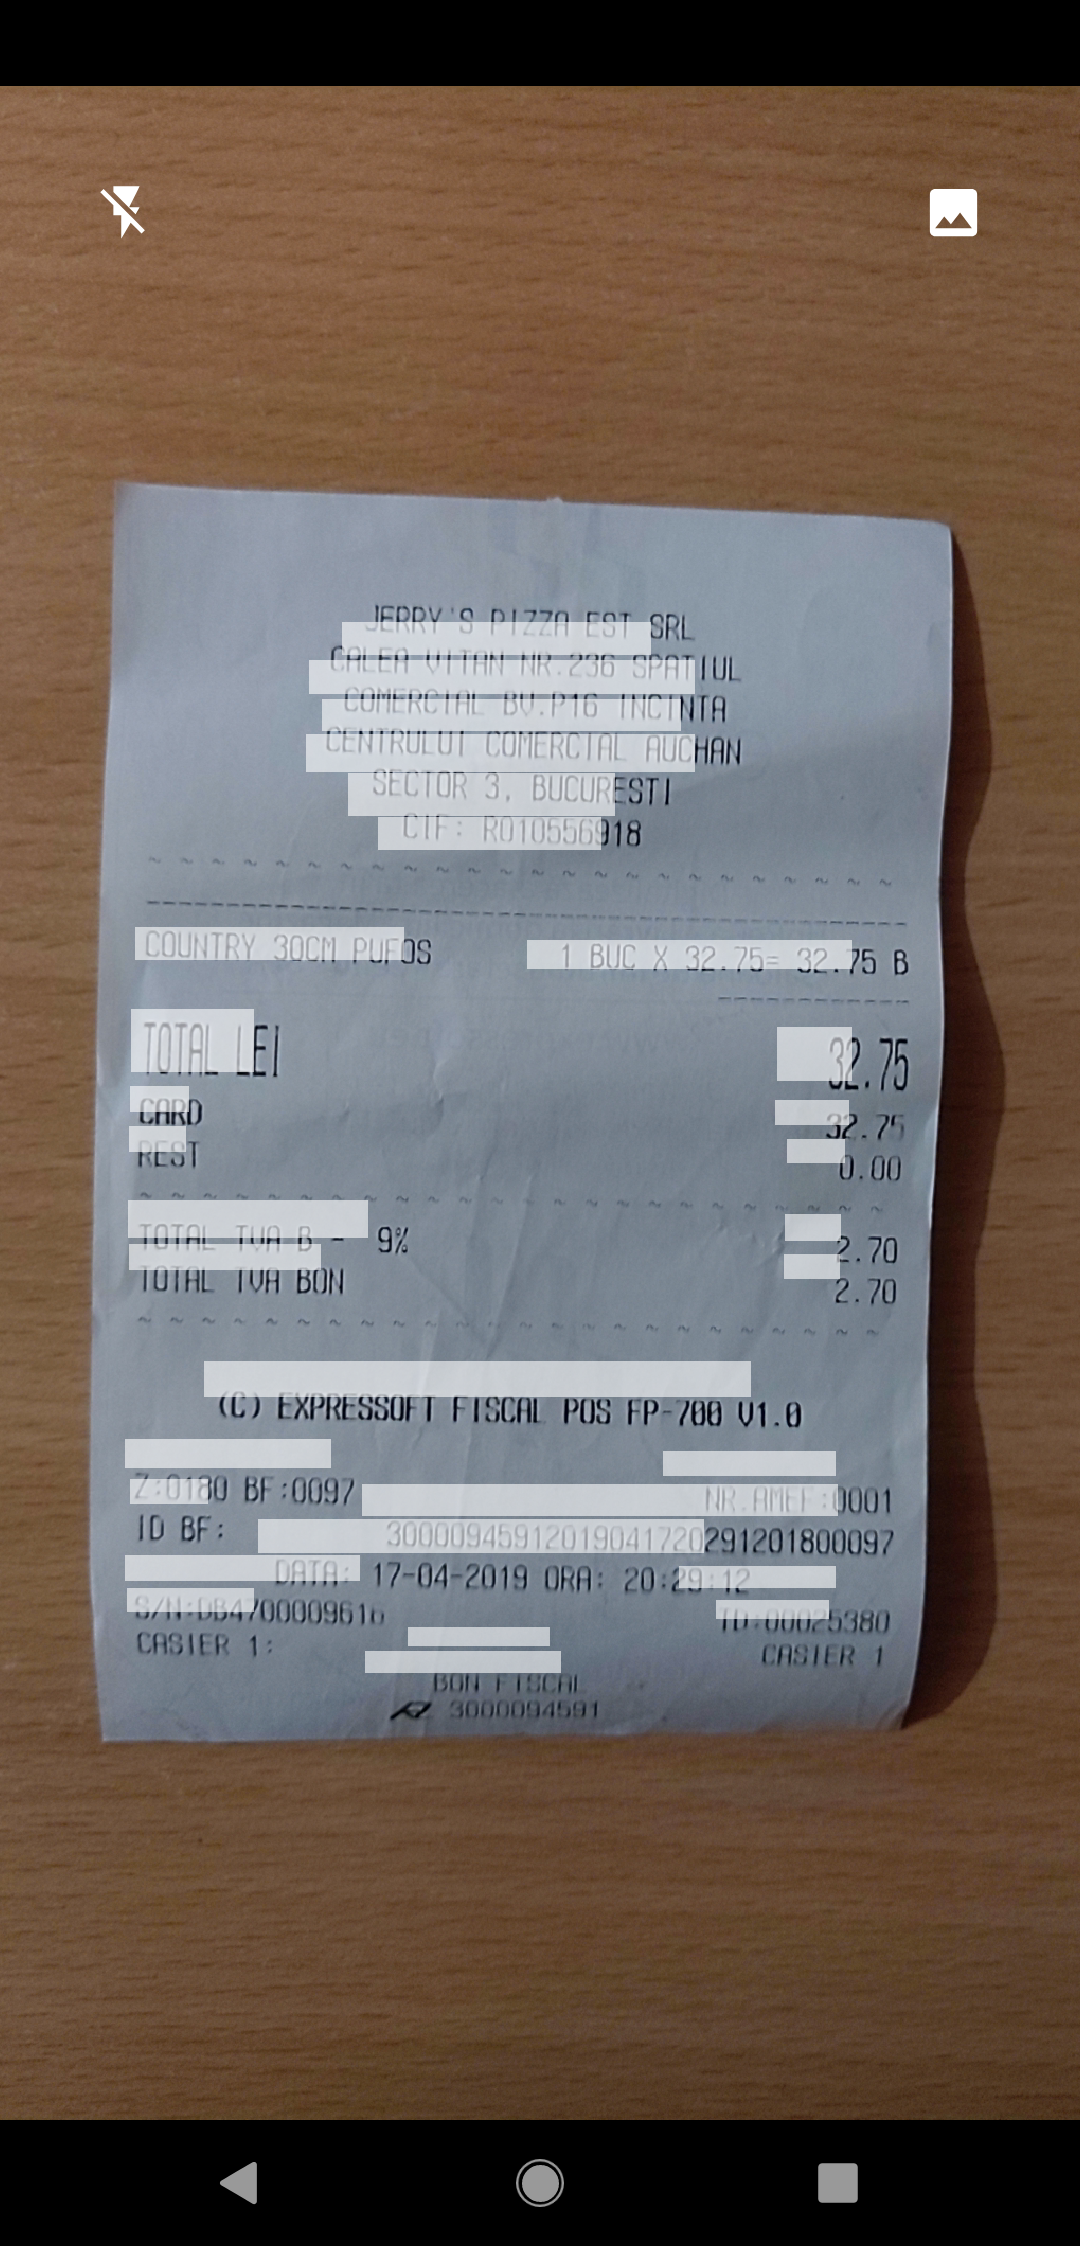
\includegraphics[width=0.25\textwidth]{Scanner.png}
%   \caption{Ecranul de Scanare}
%   \label{fig:scanner}
% \end{wrapfigure}
% \lipsum[1]


Aceasta este principala funcționalitate a aplicației și are ca scop extragerea informațiilor despre tranzacție dintr-o imagine cu un bon fiscal. Interfața cu utilizatorul este reprezentată de un vizor pentru camera principală a dispozitivului, ce afișează în timp real si textul detectat în imagine în spatele unor chenare.  Capturarea imaginii se face prin gestul \emph{tap} pe ecran. Funcționalitatea permite și folosirea unei imagini din galerie, dar și folosirea \emph{flash-ului} în condițiile de iluminare slabă. Odată capturată o imagine, procesarea acesteia se face pe un \emph{thread} secundar, în timp ce un ecran de încărcare este afișat.

\begin{figure}[ht]
  \centering
  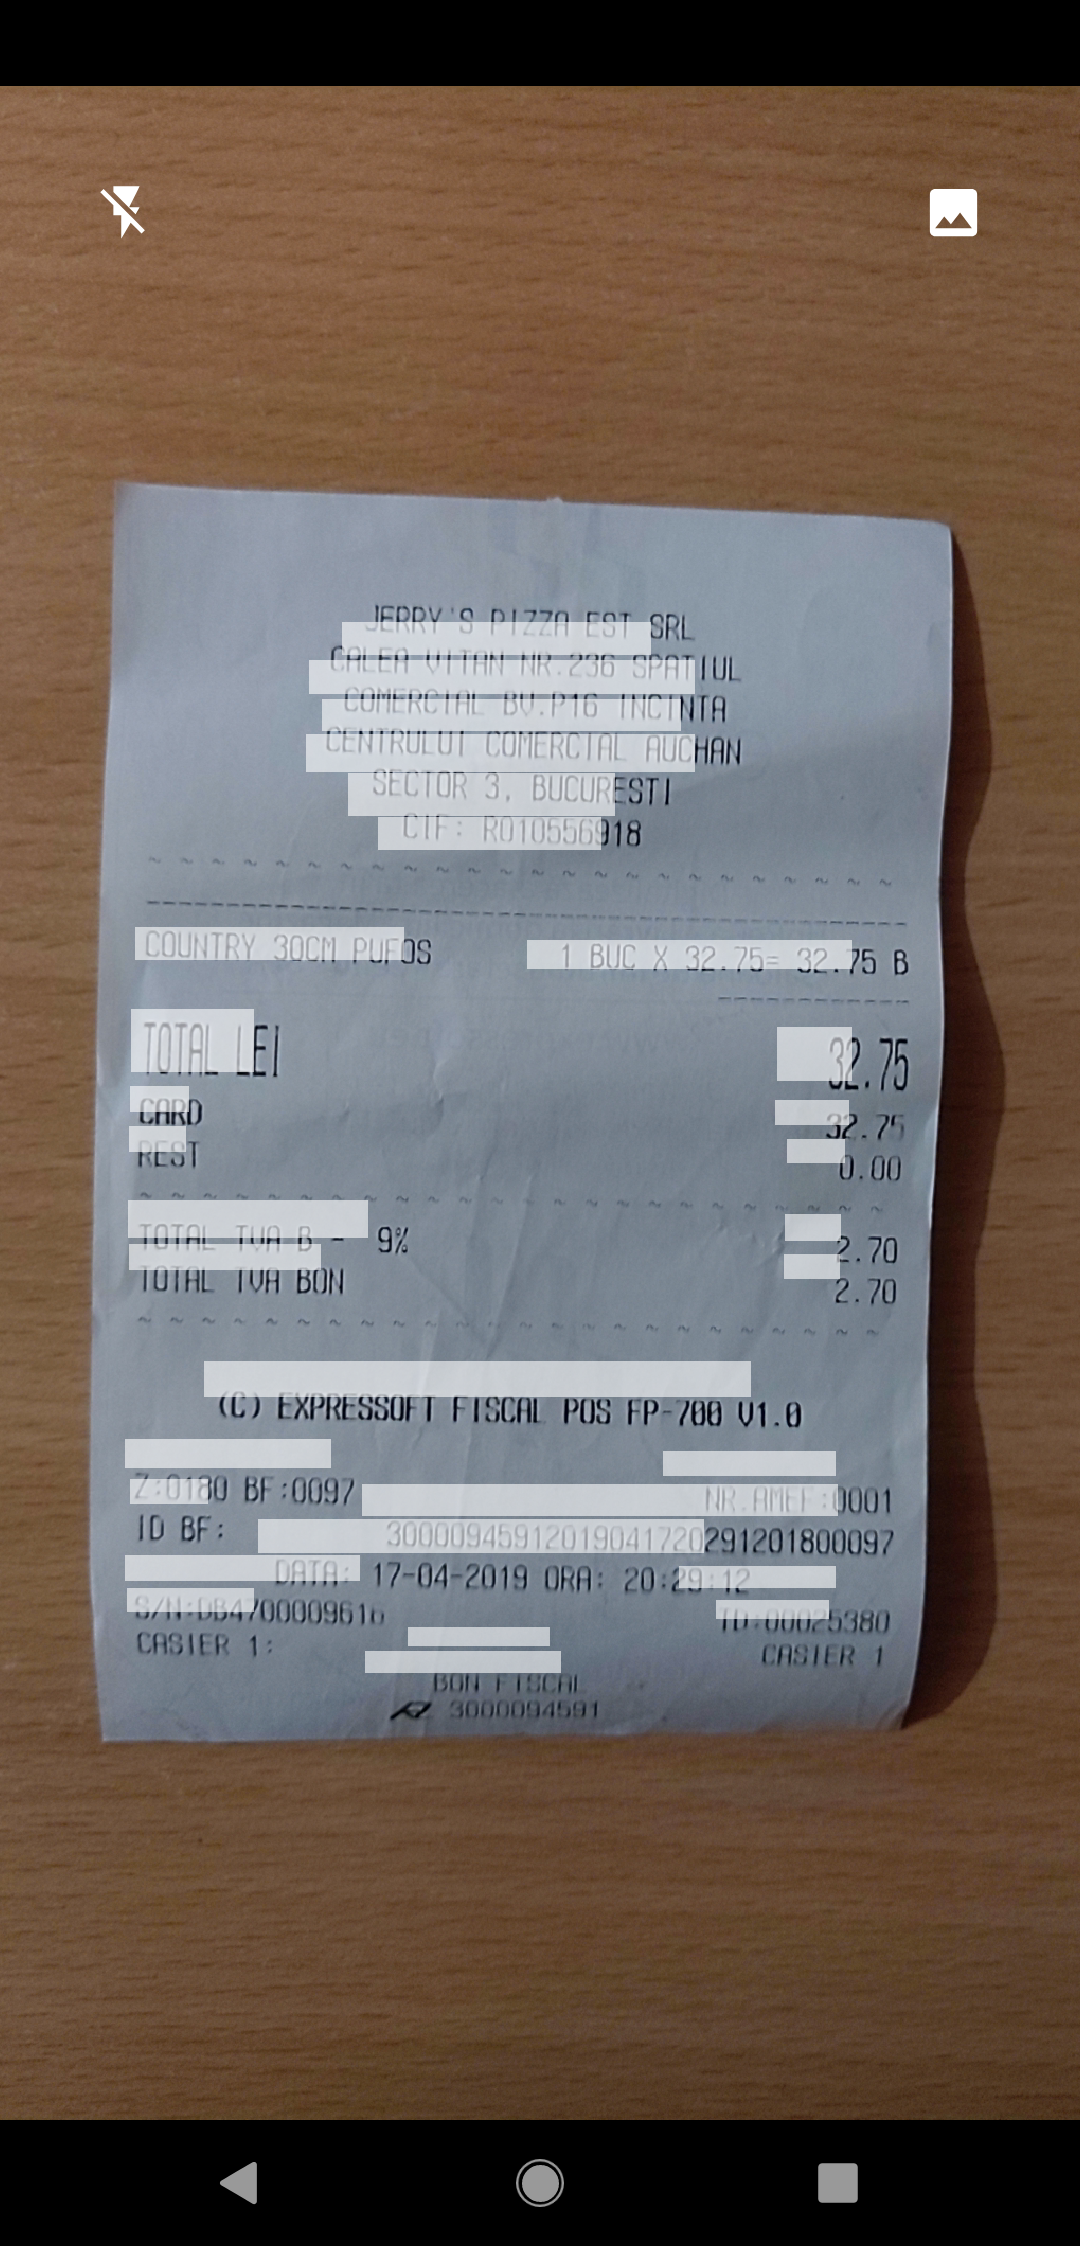
\includegraphics[width=\screenwidth]{Scanner.png}
  \caption{Ecranul de Scanare}
  \label{fig:scanner}
\end{figure}

\begin{itemize}
\item
  \textbf{Scop}: Capturarea unei imagini și extragerea informațiilor relevante din aceasta;
\item
  \textbf{Condiție de succes}: Prezența unei înregistrări în baza de date ce modelează bonul fiscal în starea de \emph{draft};
\item
  \textbf{Condiții de eșec}: Imaginea nu poate fi capturată; modulul OCR nu funcționează; o imagine este deja în curs de procesare;
\item
  \textbf{Precondiții}: Valorile predefinite pentru categorie și monedă;
\end{itemize}

\subsection*{Mențiuni}

Informațiile relevante de extras dintr-o imagine sunt:
\begin{multicols}{3}
\begin{itemize}
\item
  nume comerciant;
\item
  data tranzacției;
\item
  suma totală;
\item
  moneda;
\item
  categoria tranzacției;
\item
  produse:
  \begin{itemize}
  \item
    numele produsului;
  \item
    prețul aferent;
  \end{itemize}
\item
  elementele OCR:
  \begin{itemize}
  \item
    coordonatele casetelor de text;
  \item
    textul aferent;
  \end{itemize}
\end{itemize}
\end{multicols}

Imaginile se salvează astfel încât să nu fie accesibile din galerie.

\subsection*{Principalul scenariu}\label{principalul-scenariu}

\begin{enumerate}
\item
  Utilizatorul capturează o imagine;
\item
  Modulul OCR este apelat; Textul și chenarele aferente sunt extrase;
\item
  Rezultatul OCR este procesat pentru a obține conținutul bonului;
\item
  Bonul fiscal este salvat în stadiu de draft pentru a fi editat;
  (Editare draft)
\end{enumerate}

\subsection*{Variații}\label{variaux21bii}

\begin{itemize}
\item
  Imaginea poate fi capturată utilizând camera telefonului sau importată
  din galerie;
\item
  Moneda și categoria pot avea valori prestabilite, ce se stabilesc din
  setări; (Editare setări)
\end{itemize}

\subsection*{Extensii}\label{extensii}

\begin{itemize}
\item
  Pentru a ajuta utilizatorul atunci când folosește camera, procesarea
  imaginilor venite de la cameră se face continuu, la o rată maximă
  configurabilă;
\item
  Nu pot fi procesate mai multe imagini în același timp. Starea ultimei
  procesări este accesibilă permanent. Dacă se primește o cerere de
  procesare înainte ca ultima să se fi încheiat este semnalată o eroare.
\end{itemize}
